\subsection{B2U: Ungesteuerter Zweipuls-Gleichrichter}

% --- bestehende Grafik: Schaltung ---
\begin{center}
    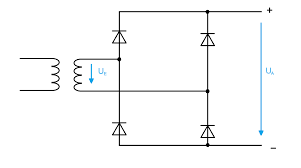
\includegraphics[width=0.85\linewidth]{images/B2U.png}
\end{center}

Der ungesteuerte Zweipuls-Gleichrichter ist eine vollwellige Brückenschaltung mit vier Dioden.
Er nutzt beide Halbwellen der Eingangsspannung und besitzt die Pulszahl $p=2$.

Eingangsspannung:
\[
u_s(t) = \hat U \sin(\omega t)
\]
mit:
\begin{itemize}
\item $\hat U$: Scheitelwert der Eingangsspannung,
\item $\omega = 2\pi f$: Kreisfrequenz,
\item $f$: Netzfrequenz.
\end{itemize}

Momentane Ausgangsspannung:
\[
u_d(t) = |u_s(t)| = |\hat U \sin(\omega t)|
\]

Mittelwert der Gleichspannung:
\[
\cbl{\overline{u_d}
= \frac{1}{\pi}\int_{0}^{\pi} \hat U \sin\gamma \, d\gamma
= \frac{2\hat U}{\pi}}
\]
mit:
\begin{itemize}
\item $\gamma = \omega t$: elektrischer Winkel.
\end{itemize}

Effektivwert der Ausgangsspannung:
\[
\cbl{U_{d,\mathrm{RMS}}
= \sqrt{\frac{1}{\pi}\int_{0}^{\pi} \hat U^2 \sin^2\gamma \, d\gamma}
= \frac{\hat U}{\sqrt{2}}}
\]

Mittelwert des Gleichstroms bei ohmscher Last $R$:
\[
\cbl{I_d = \frac{\overline{u_d}}{R} = \frac{2\hat U}{\pi R}}
\]

Effektivwert des Stroms:
\[
\cbl{I_{d,\mathrm{RMS}} = \frac{U_{d,\mathrm{RMS}}}{R}
= \frac{\hat U}{\sqrt{2}R}}
\]

Leistungsaufnahme an ohmscher Last:
\[
\cbl{P = R I_{d,\mathrm{RMS}}^2 = \frac{\hat U^2}{2R}}
\]

Restwelligkeit (Ripple-Faktor):
\[
\cbl{r = \frac{\sqrt{U_{d,\mathrm{RMS}}^2 - \overline{u_d}^2}}{\overline{u_d}}}
\]

Eigenschaften:
\begin{itemize}
\item Keine Stellmöglichkeit der Ausgangsspannung.
\item Deutlich geringere Welligkeit als beim M1U.
\item Doppelte Pulsfrequenz der Gleichspannung ($2f$).
\item Standard-Gleichrichter für einfache Anwendungen.
\end{itemize}

% --- bestehende Grafik: Spannungsverlauf ---
\begin{center}
    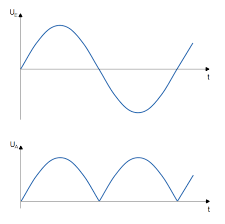
\includegraphics[width=0.85\linewidth]{images/B2U_verlauf.png}
\end{center}
\subsection{B2C: Gesteuerter Zweipuls-Gleichrichter}

% --- bestehende Grafik: Schaltung ---
\begin{center}
    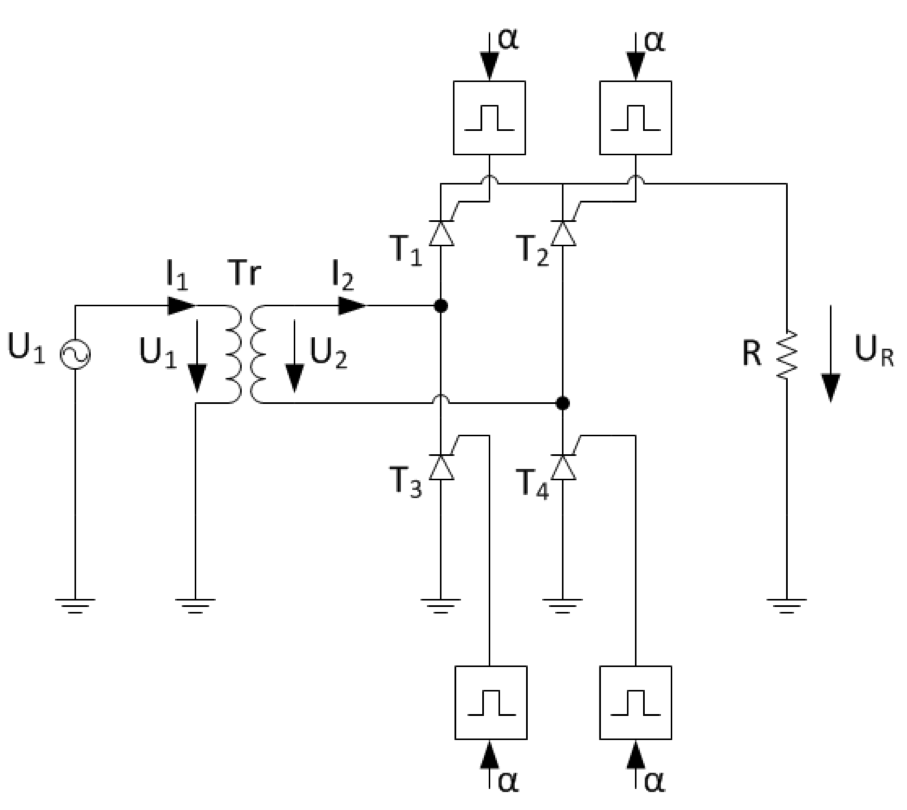
\includegraphics[width=0.85\linewidth]{images/B1C.png}
\end{center}

Der gesteuerte Zweipuls-Gleichrichter ersetzt die Dioden durch Thyristoren.
Der Leitbeginn wird über den Zündwinkel $\alpha$ gesteuert.

Eingangsspannung:
\[
u_s(t) = \hat U \sin(\omega t)
\]
mit:
\begin{itemize}
\item $\hat U$: Scheitelwert der Eingangsspannung,
\item $\omega = 2\pi f$: Kreisfrequenz,
\item $f$: Netzfrequenz.
\end{itemize}

Leitbedingung:
\[
\boxed{\omega t \ge \alpha}
\]

Momentane Ausgangsspannung:
\[
u_d(t) =
\begin{cases}
\hat U \sin(\omega t), & \omega t \ge \alpha, \\
0, & \omega t < \alpha.
\end{cases}
\]

Mittelwert der Gleichspannung:
\[
\cbl{\overline{u_d}
= \frac{1}{\pi}\int_{\alpha}^{\pi} \hat U \sin\gamma \, d\gamma
= \frac{2\hat U}{\pi}\cos\alpha}
\]

Stellbereich:
\[
0 \le \alpha \le \pi
\]

Grenzfälle:
\[
\alpha = 0 \Rightarrow \overline{u_d} = \frac{2\hat U}{\pi}
\]
\[
\alpha = \frac{\pi}{2} \Rightarrow \overline{u_d} = 0
\]
\[
\alpha > \frac{\pi}{2} \Rightarrow \overline{u_d} < 0 \quad \text{(Rückspeisebetrieb möglich)}
\]

Mittelwert des Stroms bei ohmscher Last $R$:
\[
\cbl{I_d = \frac{\overline{u_d}}{R}
= \frac{2\hat U}{\pi R}\cos\alpha}
\]

Effektivwert der Ausgangsspannung:
\[
\cbl{U_{d,\mathrm{RMS}}
= \sqrt{\frac{1}{\pi}\int_{\alpha}^{\pi} \hat U^2 \sin^2\gamma \, d\gamma}}
\]

Leistungsaufnahme an ohmscher Last:
\[
\cbl{P = R I_{d,\mathrm{RMS}}^2}
\]

Leistungsfaktor bei ohmscher Last:
\[
\cbl{\lambda = \frac{P}{U_{\mathrm{RMS}} I_{\mathrm{RMS}}}}
\]

Eigenschaften:
\begin{itemize}
\item Stellbare Gleichspannung über den Zündwinkel $\alpha$.
\item Mittelwert proportional zu $\cos\alpha$.
\item Rückspeisebetrieb für $\alpha > 90^\circ$.
\item Phasenanschnittsteuerung.
\end{itemize}

% --- bestehende Grafik: Zündwinkeldiagramm ---
\begin{center}
    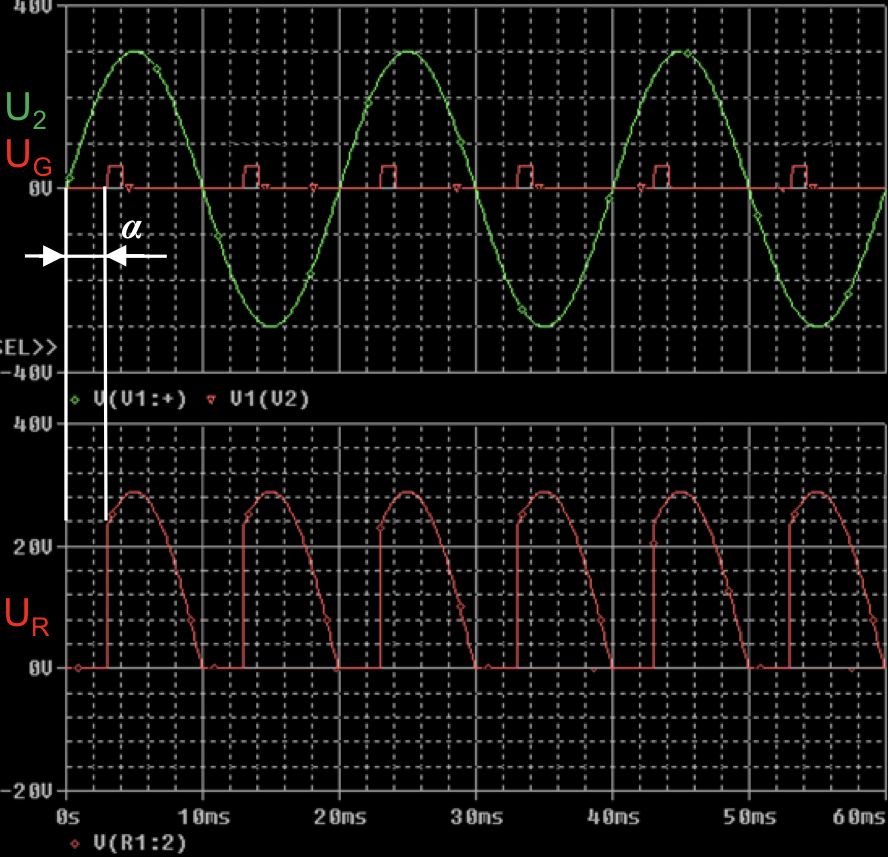
\includegraphics[width=0.85\linewidth]{images/B1C_Verlauf.png}
\end{center}
